\documentclass[11pt]{article}

\usepackage[margin=1in]{geometry}
\usepackage{amsfonts, amsmath, amssymb}
\usepackage[none]{hyphenat}
\usepackage{fancyhdr}
\usepackage{graphicx}
\usepackage{float}
\usepackage[nottoc, notlot, notlof]{tocbibind}
\usepackage{hyperref}

\pagestyle{fancy}
\fancyhead{}
\fancyfoot{}
\fancyhead[L]{\slshape \MakeUppercase{Cassette deck}}
\fancyhead[R]{\slshape Diagrams}
\fancyfoot[C]{\thepage}
\renewcommand{\footrulewidth}{0pt}

\parindent 0ex %
\renewcommand{\baselinestretch}{1.5}

\begin{document}

\begin{titlepage}
\begin{center}
\vspace*{1cm}
\Large{\textbf{Software Engineering}}\\
\Large{\textbf{Modeling and Implementation Project}}
\vfill
\line(1,0){400}\\[1mm]
\huge{\textbf{“Simulator of a Cassette Deck”}}\\[3mm]
\Large{\textbf{- Diagrams -}}\\[1mm]
\line(1,0){400}\\
\vfill
By Constant Théo and Essafsyfy Abdelkrim\\
Academic year 2018-2019
\end{center}
\end{titlepage}

\tableofcontents
\thispagestyle{empty}
\clearpage
\setcounter{page}{1}

\section{Use case diagram}
\subsection{Diagram}
\vspace{10px}
\begin{center}
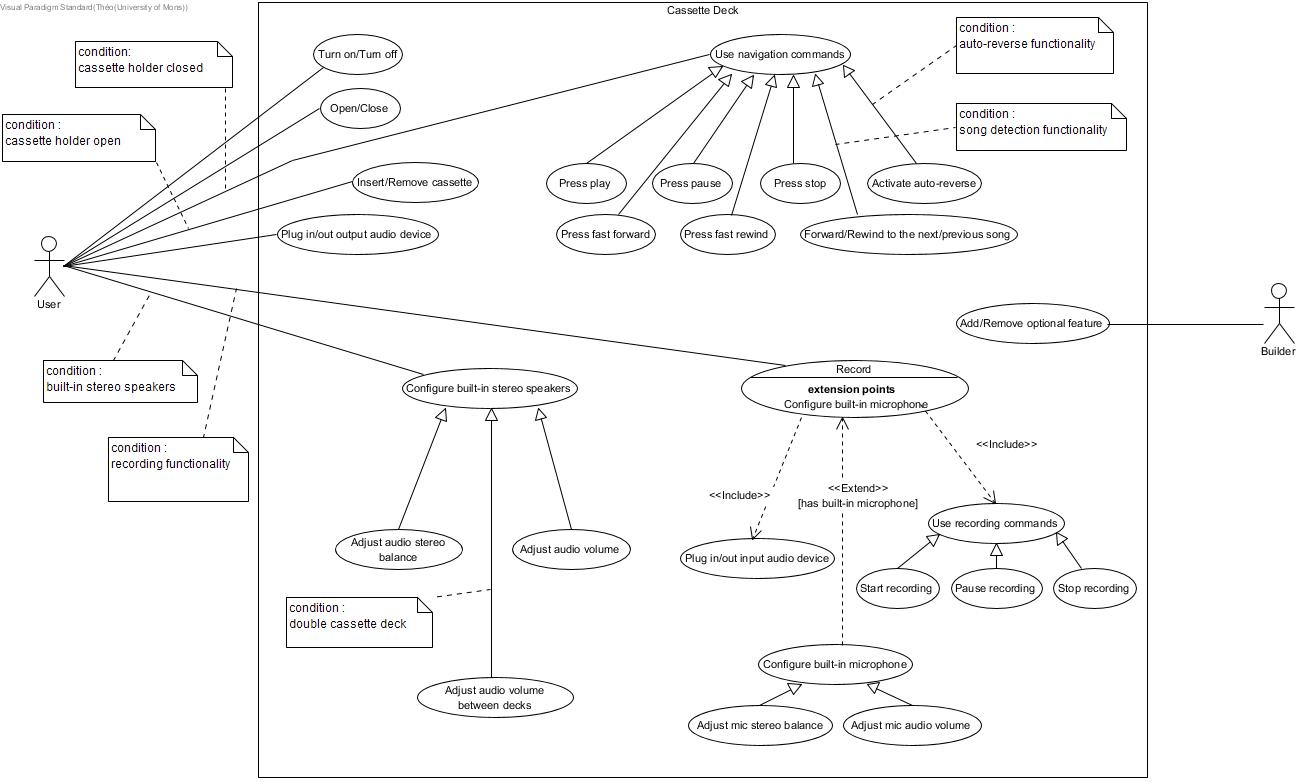
\includegraphics[width=15cm]{./img/useCaseD.jpg}\\
\end{center}

\subsection{Cases' description}
\subsubsection{Turn on/Turn off}
\textbf{Use case name} : Turn on/Turn off\\
\textbf{Summary} : Allows the user to turn the cassette deck on or off.\\
\textbf{Actors} : User.\\
\textbf{Assumptions} :Cassette deck has access to a power source.\\
\textbf{Preconditions} : Cassette holder is closed\\
\textbf{Basic course of action :}\\
1. User presses power button on.\\
2. Cassette deck is powered on.\\
\textbf{Postconditions} : Same as preconditions.\\
\textbf{Alternate courses :}\\
2a : Cassette deck is powered off.\\

\subsubsection{Open/Close}
\textbf{Use case name} : Open/Close\\
\textbf{Summary} : Allows the user to open or closes the cassette holder.\\
\textbf{Actors} : User.\\
\textbf{Assumptions} :Cassette deck is plugged in.\\
\textbf{Preconditions} : Cassette deck is powered on.\\
\textbf{Basic course of action :}\\
1. User presses eject button.\\
2. Cassette holder opens.\\
\textbf{Postconditions} : Same as preconditions.\\
\textbf{Alternate courses :}\\
2b : Cassette holder closes.\\

\subsubsection{Insert/Remove cassette}
\textbf{Use case name} : Insert/Remove cassette\\
\textbf{Summary} : Allows the user to insert or remove a cassette from the cassette holder\\
\textbf{Actors} : User.\\
\textbf{Assumptions} :Cassette deck is powered on.\\
\textbf{Preconditions} : Cassette holder is open.\\
\textbf{Basic course of action :}\\
1. User presses eject button.\\
2. Cassette holder opens.\\
3. User inserts a cassette into the cassette holder.\\
\textbf{Postconditions} : Cassette holder is closed\\
\textbf{Alternate courses :}\\
3a : User removes a cassette from the cassette holder.\\

\subsubsection{Plug in/out audio device}
\textbf{Use case name} : Plug in/out audio device\\
\textbf{Summary} : Allows user to plug in or out an external audio device\\
\textbf{Actors} : User.\\
%\textbf{Preconditions} :\\
\textbf{Basic course of action :}\\
1. User plugs in an external audio device.\\
\textbf{Alternate courses :}\\
1a : User plugs out an external audio device.\\

\subsubsection{Use navigation commands}
\textbf{Use case name} : Use navigation commands\\
\textbf{Summary} : An abstract use case containing common sub classes descriptions.\\
\textbf{Actors} : User\\
\textbf{Assumptions} :Cassette deck is powered on.\\
\textbf{Preconditions} : Cassette inserted into the deck.\\

\subsubsection{Press play}
\textbf{Use case name} : Press play\\
\textbf{Summary} : Allows the user to press play button to play music.\\
\textbf{Actors} : Same as parent use-case.\\
\textbf{Assumptions} : Same as parent use-case\\
\textbf{Preconditions} :Magnetic head engaged and cassette deck must be in idle state\\
\textbf{Basic course of action :}\\
1. User presses play button.\\
2. Magnetic head engages.\\
3. Music starts playing.\\
\textbf{Postconditions} : Magnetic head disengaged\\

\subsubsection{Press pause}
\textbf{Use case name} : Press pause\\
\textbf{Summary} : Allows the user to press pause button to pause music.\\
\textbf{Actors} : Same as parent use-case.\\
\textbf{Assumptions} : Same as parent use-case.\\
\textbf{Preconditions} : Same as parent use-case and Magnetic head engaged.\\
\textbf{Basic course of action :}\\
1. User presses pause button.\\
2. Music pauses playing.\\
\textbf{Postconditions} : Magnetic head disengaged\\

\subsubsection{Press stop}
\textbf{Use case name} : Press stop\\
\textbf{Summary} : Allows the user to press stop button to stop music.\\
\textbf{Actors} : Same as parent use-case.\\
\textbf{Assumptions} : Same as parent use-case\\
\textbf{Preconditions} : Same as parent use-case.\\
%\textbf{Preconditions} :Magnetic head disengaged.\\
\textbf{Basic course of action :}\\
1. User presses play button.\\
2. Magnetic head disengages.\\
3. Music stops playing.\\

\subsubsection{Press fast forward}
\textbf{Use case name} : Press fast forward\\
\textbf{Summary} : Allows the user to press fast forward button\\
\textbf{Actors} : Same as parent use-case.\\
\textbf{Assumptions} : Same as parent use-case.\\
\textbf{Preconditions} :Same as parent use-case, magnetic head disengaged and cassette deck must be in idle state\\
\textbf{Basic course of action :}\\
1. User presses fast forward button.\\
2. Magnetic head disengages.\\
3. Music is fast forwarded.\\
\textbf{Postconditions} : Magnetic head disengaged\\

\subsubsection{Press fast rewind}
\textbf{Use case name} : Press fast rewind\\
\textbf{Summary} : Allows the user to press fast rewind button.\\
\textbf{Actors} : Same as parent use-case.\\
\textbf{Assumptions} : Same as parent use-case.\\
\textbf{Preconditions} : Same as parent use-case, magnetic head disengaged and cassette deck must be in idle state\\
\textbf{Basic course of action :}\\
1. User presses fast rewind button.\\
2. Magnetic head disengages.\\
3. Music is fast re-winded.\\
\textbf{Postconditions} : Magnetic head disengaged\\

\subsubsection{Forward/Rewind to the next/previous song}
\textbf{Use case name} : Forward/Rewind to the next/previous song\\
\textbf{Summary} : \\
\textbf{Actors} : Same as parent use-case.\\
\textbf{Assumptions} : Same as parent use-case.\\
\textbf{Preconditions} :Same as parent use-case, magnetic head disengaged, and cassette deck must be in idle state\\
\textbf{Basic course of action :}\\
1. User presses forward to next song.
2. Deck fast forwards to the next song.
3. Return to idle state.
\textbf{Postconditions} : \\
\textbf{Alternate courses :}\\
1a. User presses rewind to previous song.\\
2a. Deck fast rewinds to the previous song.\\

\subsubsection{Activate auto-reverse}
\textbf{Use case name} : Activate auto-reverse\\
\textbf{Summary} : Allows the user to press auto-reverse button.\\
\textbf{Actors} : Same as parent use-case.\\
\textbf{Assumptions} : Same as parent use-case.\\
\textbf{Preconditions} : Same as parent use-case and deck has an auto-reverse functionality\\
\textbf{Basic course of action :}\\
1. User presses auto-reverse button.\\
2. Magnetic head reaches the end of the tape.\\
3. Magnetic head on one side disengages.\\
4. Magnetic head on the other engages.\\

\subsubsection{Configure built-in stereo speakers}
\textbf{Use case name} : Configure built-in stereo speakers\\
\textbf{Summary} : An abstract use case containing common sub classes descriptions.\\
\textbf{Actors} : User\\
\textbf{Assumptions} :Cassette deck is powered on.\\
\textbf{Preconditions} : Built-in stereo speaker\\

\subsubsection{Adjust audio stereo balance}
\textbf{Use case name} : Adjust audio stereo balance\\
\textbf{Summary} : Allows the user to adjust the audio stereo balance of the deck\\
\textbf{Actors} : Same as parent use-case.\\
\textbf{Assumptions} : Same as parent use-case.\\
\textbf{Preconditions} : Same as parent use-case.\\
\textbf{Basic course of action :}\\
1. User turns audio stereo balance knob\\
2. Audio stereo balance increases\\
\textbf{Alternate courses :}\\
2a : Audio stereo balance decreases\\

\subsubsection{Adjust audio volume}
\textbf{Use case name} : Adjust audio volume\\
\textbf{Summary} : Allows the user to adjust the audio volume of the deck\\
\textbf{Actors} : Same as parent use-case.\\
\textbf{Assumptions} : Same as parent use-case.\\
\textbf{Preconditions} : Same as parent use-case.\\
\textbf{Basic course of action :}\\
1. User turns audio volume balance knob\\
2. Audio volume increases\\
%\textbf{Postconditions} : \\
\textbf{Alternate courses :}\\
2a : Audio volume decreases\\

\subsubsection{Adjust audio volume between decks}
\textbf{Use case name} : Adjust audio volume between decks\\
\textbf{Summary} : Allows the user to adjust the audio volume of two decks\\
\textbf{Actors} : Same as parent use-case.\\
\textbf{Assumptions} : Same as parent use-case.\\
\textbf{Preconditions} : Same as parent use-case and double cassette deck\\
\textbf{Basic course of action :}\\
1. User turns audio volume balance knob\\
2. Audio volume increases\\
%\textbf{Postconditions} : \\
\textbf{Alternate courses :}\\
2a : Audio volume decreases\\

\subsubsection{Record}
\textbf{Use case name} : Record\\
\textbf{Summary} : Allows the user to record audio using a microphone\\
\textbf{Actors} : User\\
\textbf{Assumptions} :Cassette deck is plugged in.\\
\textbf{Preconditions} : Recording functionality available\\
\textbf{Basic course of action :}\\
1. User presses the record button.\\
2. Deck starts recording audio.\\
\textbf{Postconditions} : Same as preconditions.\\

\subsubsection{Plug in/out input audio device}
\textbf{Use case name} : Plug in/out input audio device\\
\textbf{Summary} : Allows the user to plug in or out an input audio device to the deck\\
\textbf{Actors} : User\\
\textbf{Assumptions} : Cassette deck in turned on.\\
\textbf{Preconditions} : \\
\textbf{Basic course of action :}\\
1. User plugs in an in input audio device.\\
\textbf{Postconditions} : Same as preconditions.\\
\textbf{Alternate courses :}\\
1. User plugs out an in input audio device.\\

\subsubsection{Configure built-in microphone}
\textbf{Use case name} :Configure built-in microphone\\
\textbf{Summary} : An abstract use case that allows the user to configure a built-in microphone\\
\textbf{Actors} : User\\
\textbf{Assumptions} : Cassette deck in turned on.\\
\textbf{Preconditions} : Built-in microphone\\
\textbf{Basic course of action :}\\
1. User configures a built-in microphone.\\
\textbf{Postconditions} : Same as preconditions.\\

\subsubsection{Adjust mic stereo balance}
\textbf{Use case name} : Adjust mic stereo balance\\
\textbf{Summary} : Allows the user to adjust deck's mic stereo balance\\
\textbf{Actors} : Same as parent.\\
\textbf{Assumptions} : Same as parent.\\
\textbf{Preconditions} : Same as parent.\\
\textbf{Basic course of action :}\\
1. User adjust mic stereo balance.\\
\textbf{Postconditions} : Same as parent.\\

\subsubsection{Adjust mic audio volume}
\textbf{Use case name} : Adjust mic audio volume\\
\textbf{Summary} : Allows the user to adjust deck's audio volume\\
\textbf{Actors} : Same as parent.\\
\textbf{Assumptions} : Same as parent.\\
\textbf{Preconditions} : Same as parent.\\
\textbf{Basic course of action :}\\
1. User adjust audio volume.\\
\textbf{Postconditions} : Same as parent.\\

\subsubsection{Adjust mic audio volume}
\textbf{Use case name} : Adjust mic audio volume\\
\textbf{Summary} : Allows the user to adjust deck's audio volume\\
\textbf{Actors} : Same as parent.\\
\textbf{Assumptions} : Same as parent.\\
\textbf{Preconditions} : Same as parent.\\
\textbf{Basic course of action :}\\
1. User adjust audio volume.\\
\textbf{Postconditions} : Same as parent.\\

\subsubsection{Use recording commands}
\textbf{Use case name} : Use recording commands\\
\textbf{Summary} : An abstract use case that allows the user to use recording commands\\
\textbf{Actors} : User\\
\textbf{Assumptions} : Cassette deck in turned on.\\
\textbf{Preconditions} : Built-in microphone\\
%\textbf{Basic course of action :}\\
\textbf{Postconditions} : Same as preconditions.\\
%\textbf{Alternate courses :}\\

\subsubsection{Start recording}
\textbf{Use case name} : Start recording\\
\textbf{Summary} : Allows the user to start recording audio\\
\textbf{Actors} : Same as parent.\\
\textbf{Assumptions} : Same as parent.\\
\textbf{Preconditions} : Same as parent.\\
\textbf{Basic course of action :}\\
1. User presses the start recording button.\\
2. Deck starts recording audio.\\
\textbf{Postconditions} : Same as parent.\\
%\textbf{Alternate courses :}\\

\subsubsection{Pause recording}
\textbf{Use case name} : Pause recording\\
\textbf{Summary} : Allows the user to pause recording audio\\
\textbf{Actors} : Same as parent.\\
\textbf{Assumptions} : Same as parent.\\
\textbf{Preconditions} : Same as parent.\\
\textbf{Basic course of action :}\\
1. User presses the pause recording button.\\
2. Deck pauses recording audio.\\
\textbf{Postconditions} : Same as parent.\\
%\textbf{Alternate courses :}\\

\subsubsection{Stop recording}
\textbf{Use case name} : Stop recording\\
\textbf{Summary} : Allows the user to stop recording audio\\
\textbf{Actors} : Same as parent.\\
\textbf{Assumptions} : Same as parent.\\
\textbf{Preconditions} : Same as parent.\\
\textbf{Basic course of action :}\\
1. User presses the stop recording button.\\
2. Deck stops recording audio.\\
\textbf{Postconditions} : Same as parent.\\
%\textbf{Alternate courses :}\\


\pagebreak
\section{Class diagram}
\vspace{10px}
\begin{center}
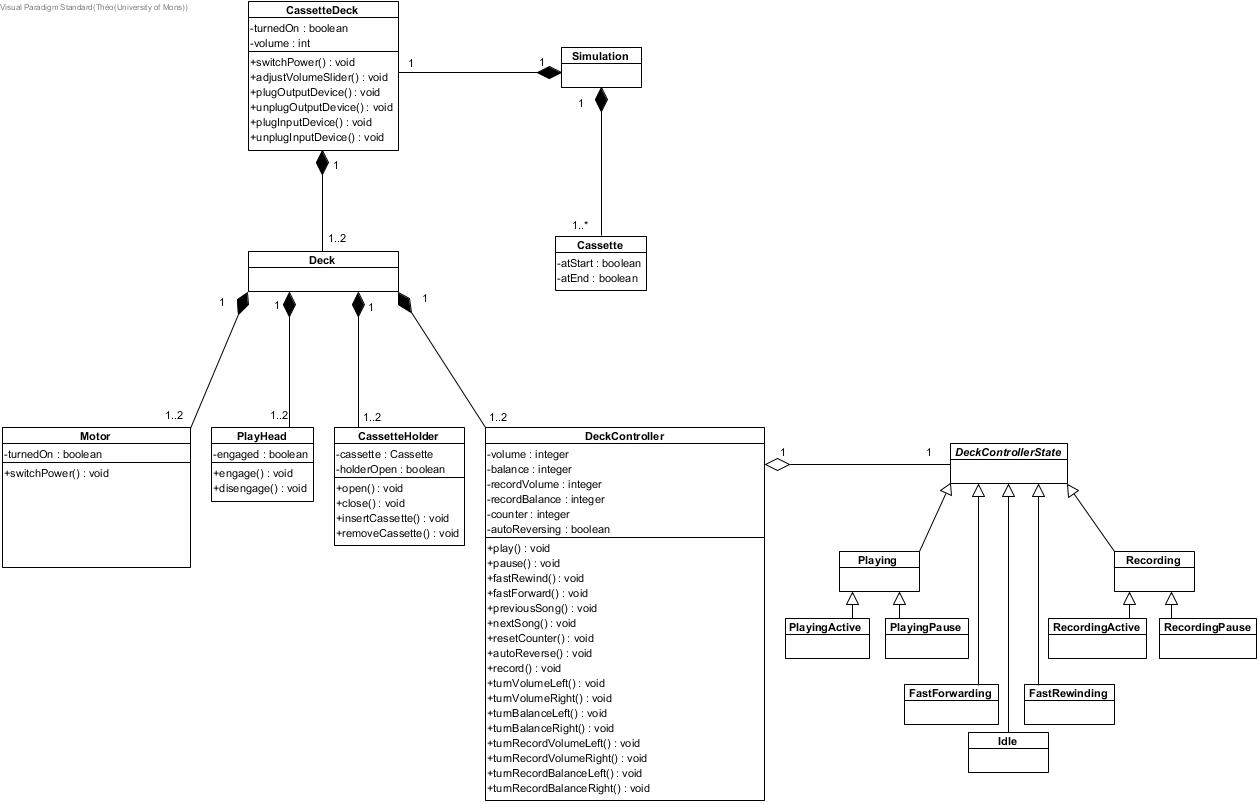
\includegraphics[width=15cm]{./img/class_diagram.jpg}\\
\end{center}
This diagram shows the different classes we’ll use in the implementation.
First, we can see a Simulation class : it corresponds to a simulation session and contains one CassetteDeck object and one or several Cassette objects.
The Cassette class allows us to instanciate cassettes, with possibly an audio file in them.\\
The CassetteDeck class is the device itself. It handles the general buttons like the power button or the volume slider. It contains one or two Deck objects, according to the type of device (some are double cassette decks). Each Deck contains a Motor, a CassetteHolder and a DeckController object, and one or two PlayHead objects (two if it has an auto-reverse functionality).\\
The DeckController class is the most important class for the user : it contains almost all the commands he can perform, like play, stop or fastRewind. This object can have differents states. Therefore, we have decided to implement the state design pattern for it. The class contains an abstract DeckControllerState class, whose inherit seven possible states. Playing and Recording are also abstract. According to the state design pattern, all those classes have the same operations than DeckController (for some clarity, we didn’t write them on the diagram).


\pagebreak
\section{State Charts Diagrams \textit{(Yakindu)}}
\subsection{Diagram 1}
\vspace{10px}
\begin{center}
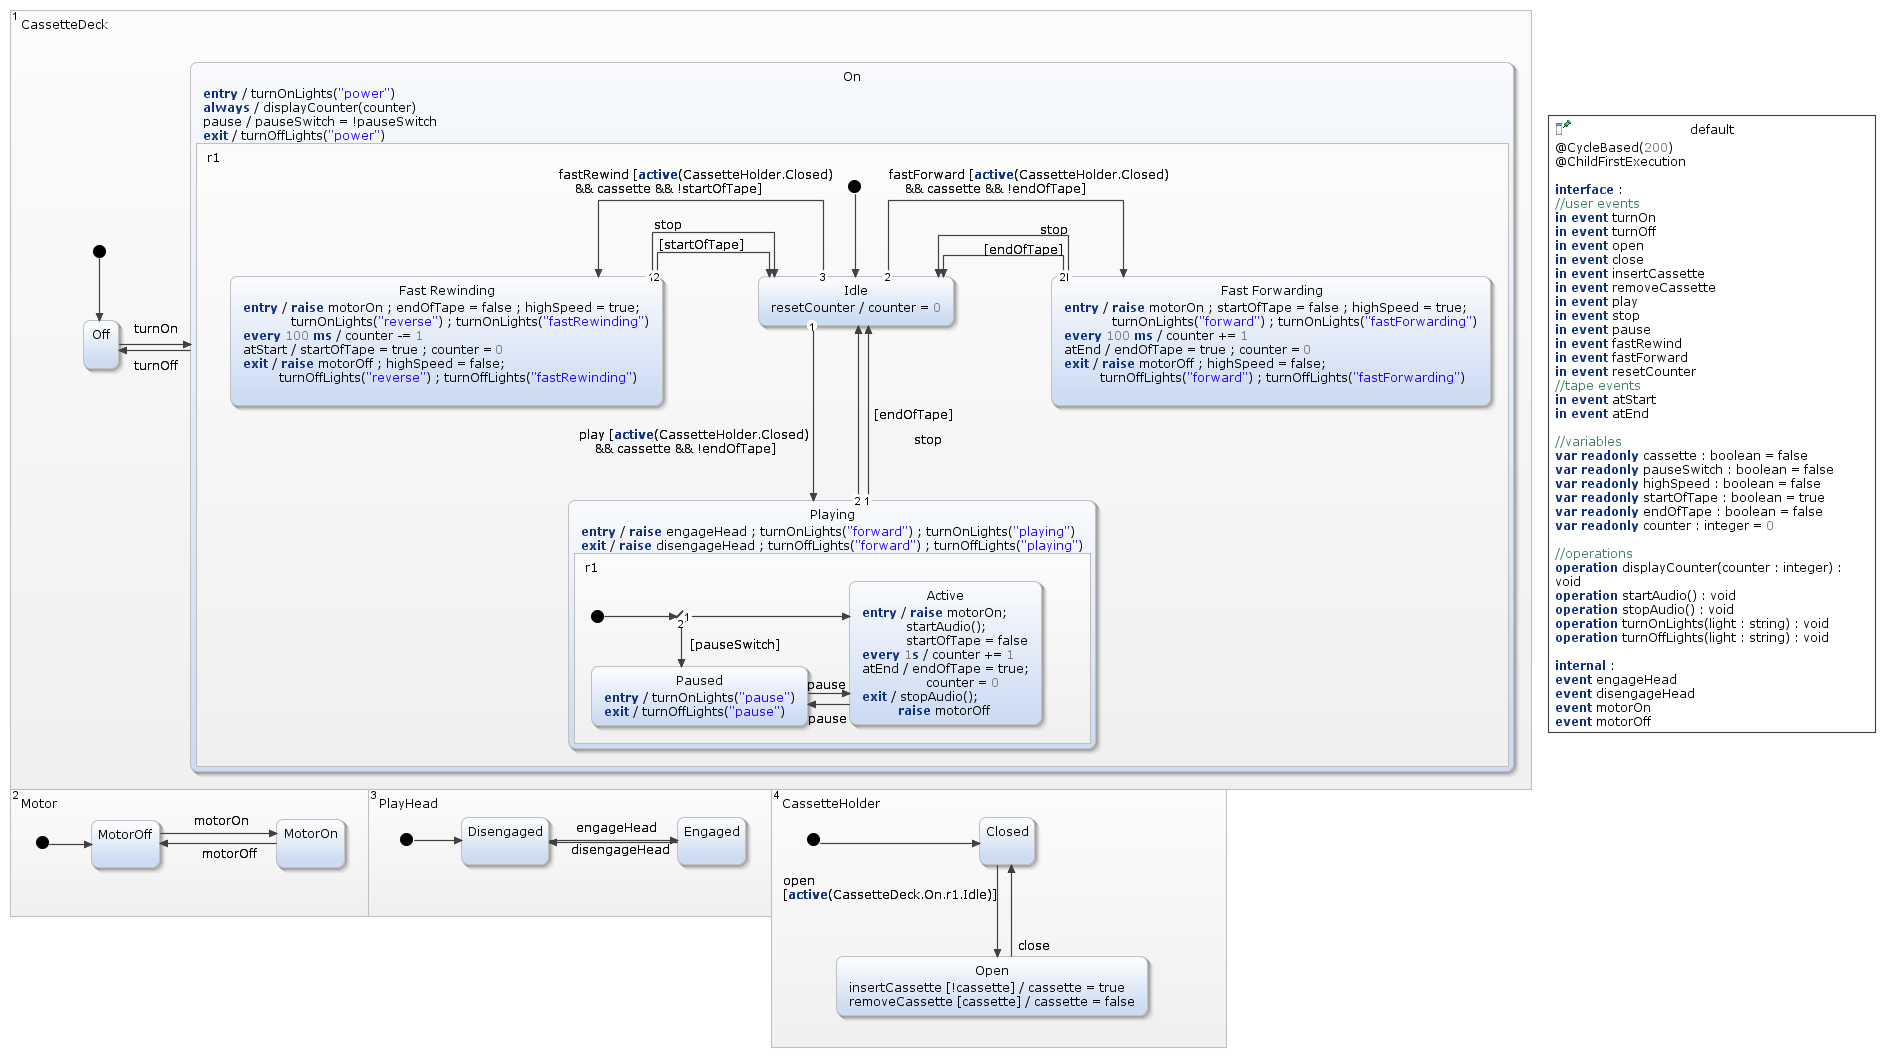
\includegraphics[width=15cm]{./img/statechart_diagram1.png}\\
\end{center}


\subsection{Diagram 2}
\vspace{10px}
\begin{center}
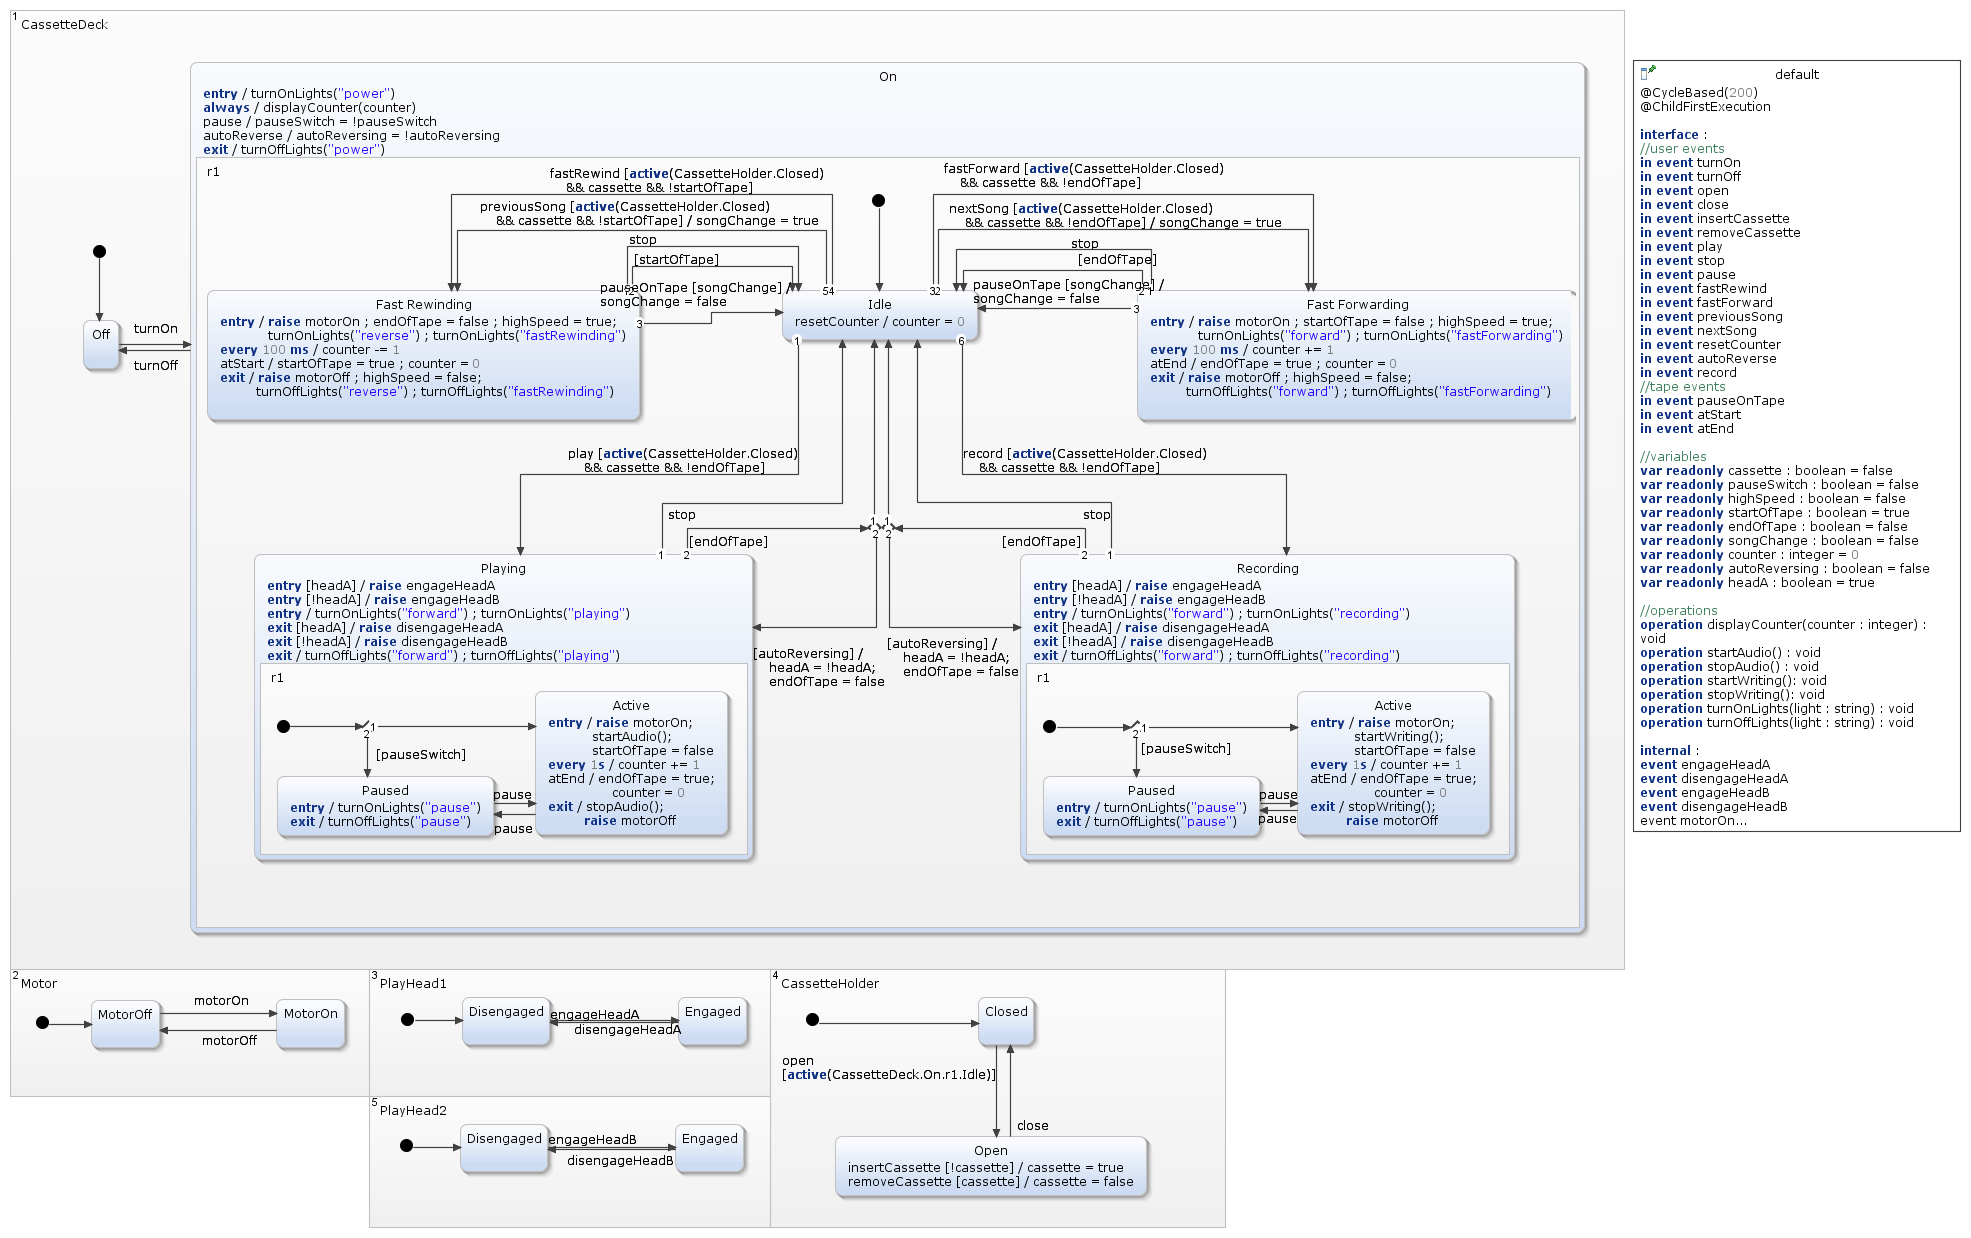
\includegraphics[width=15cm]{./img/statechart_diagram2.png}\\
\end{center}


\subsection{Diagram 3}
\vspace{10px}
\begin{center}
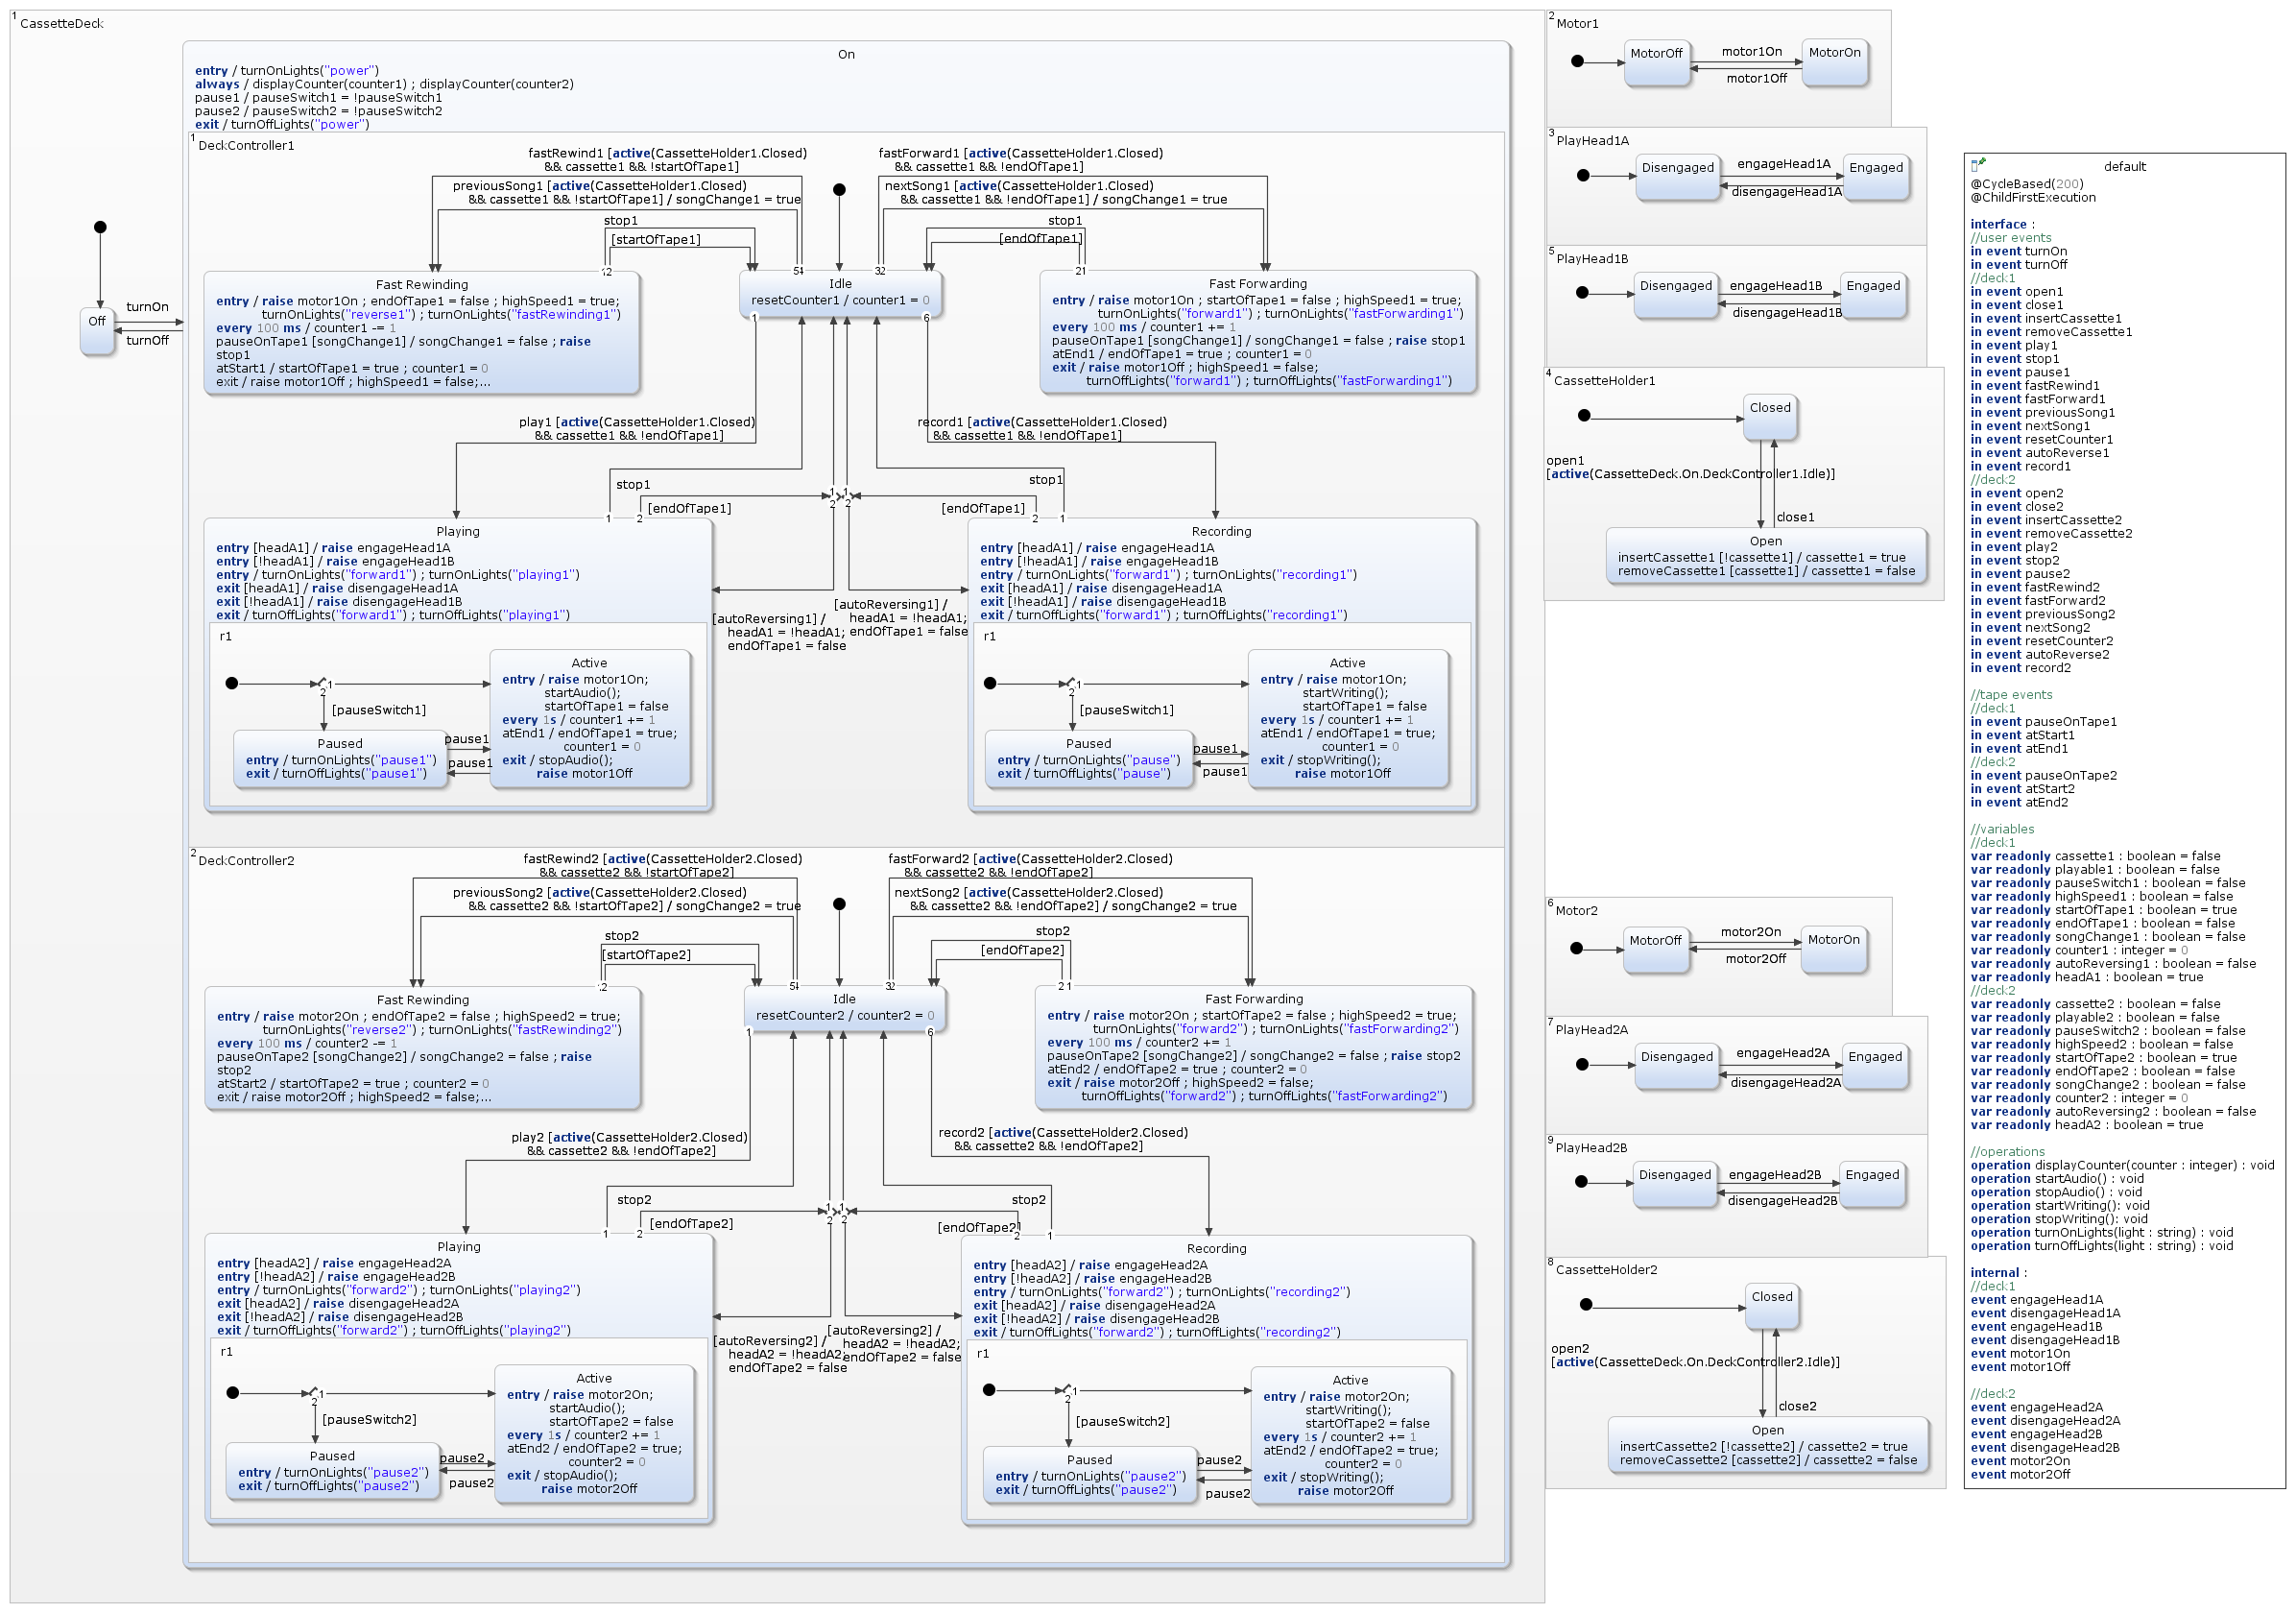
\includegraphics[width=15cm]{./img/statechart_diagram3.png}\\
\end{center}

Those diagrams show all the different states in the application and their relations, for a simple cassette deck, a more complex one, and finally a double cassette deck.
This last diagram is the most complete one, so this is the one we’ll be describing here.\\
There is a CassetteDeck region, that is separated in two concurrent states, for the two decks. There are also a Motor region, two PlayHead regions and a CassetteHolder region for each deck. Those two decks are living separately, so the user can record the other one while it is playing a cassette.
When the user turns the cassette deck on, the object enters in the "On" state. Each deck starts in the "Idle" state, and this is the central state: the deck has to be in this state before entering most of the other states.\\
Playing and Recording states contain Paused and Active states. The pause button is a switch button and can be switched at any time, unlike the other buttons.

\pagebreak
\section{Sequence diagrams}
The sequence diagram describes the interactions between its components, it also formalizes the behavior described by the Use case diagram.\\
In this instance, we used two example diagrams to describe this behavior; Music player and Music recorder.
\subsection{Music Player}
\vspace{10px}
\begin{center}
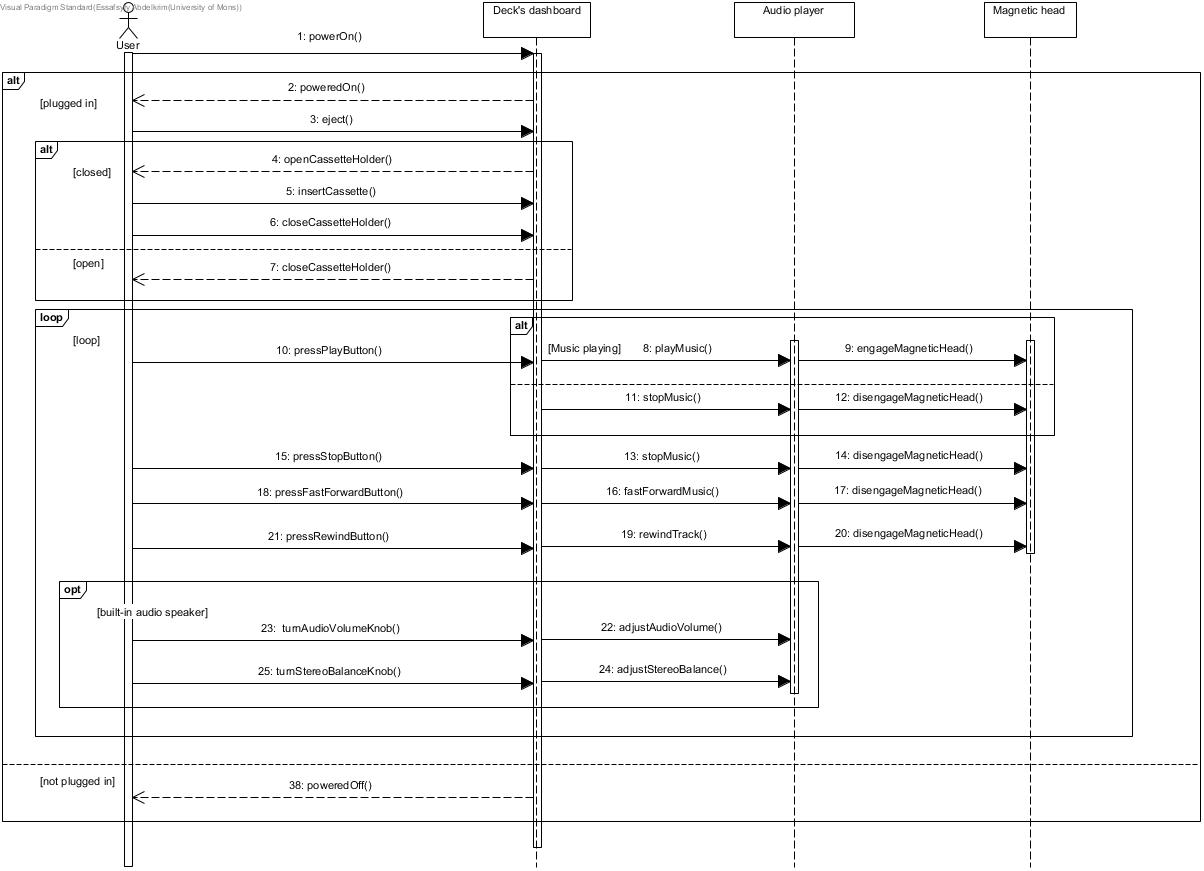
\includegraphics[width=15cm]{./img/musicPlayer(SD).jpg}\\
\end{center}
This diagram describes the steps a user follows to play, pause, stop, fast forward or rewind music using the deck's dashboard. All these features can be looped, thus allowing the user to play, pause then play, for instance. If the deck has a built-in audio speaker, the user is able to adjust the audio volume and the stereo balance using the respective knob. All operations are only feasible if the deck is plugged in to a power source.

\subsection{Music Recorder}
\vspace{10px}
\begin{center}
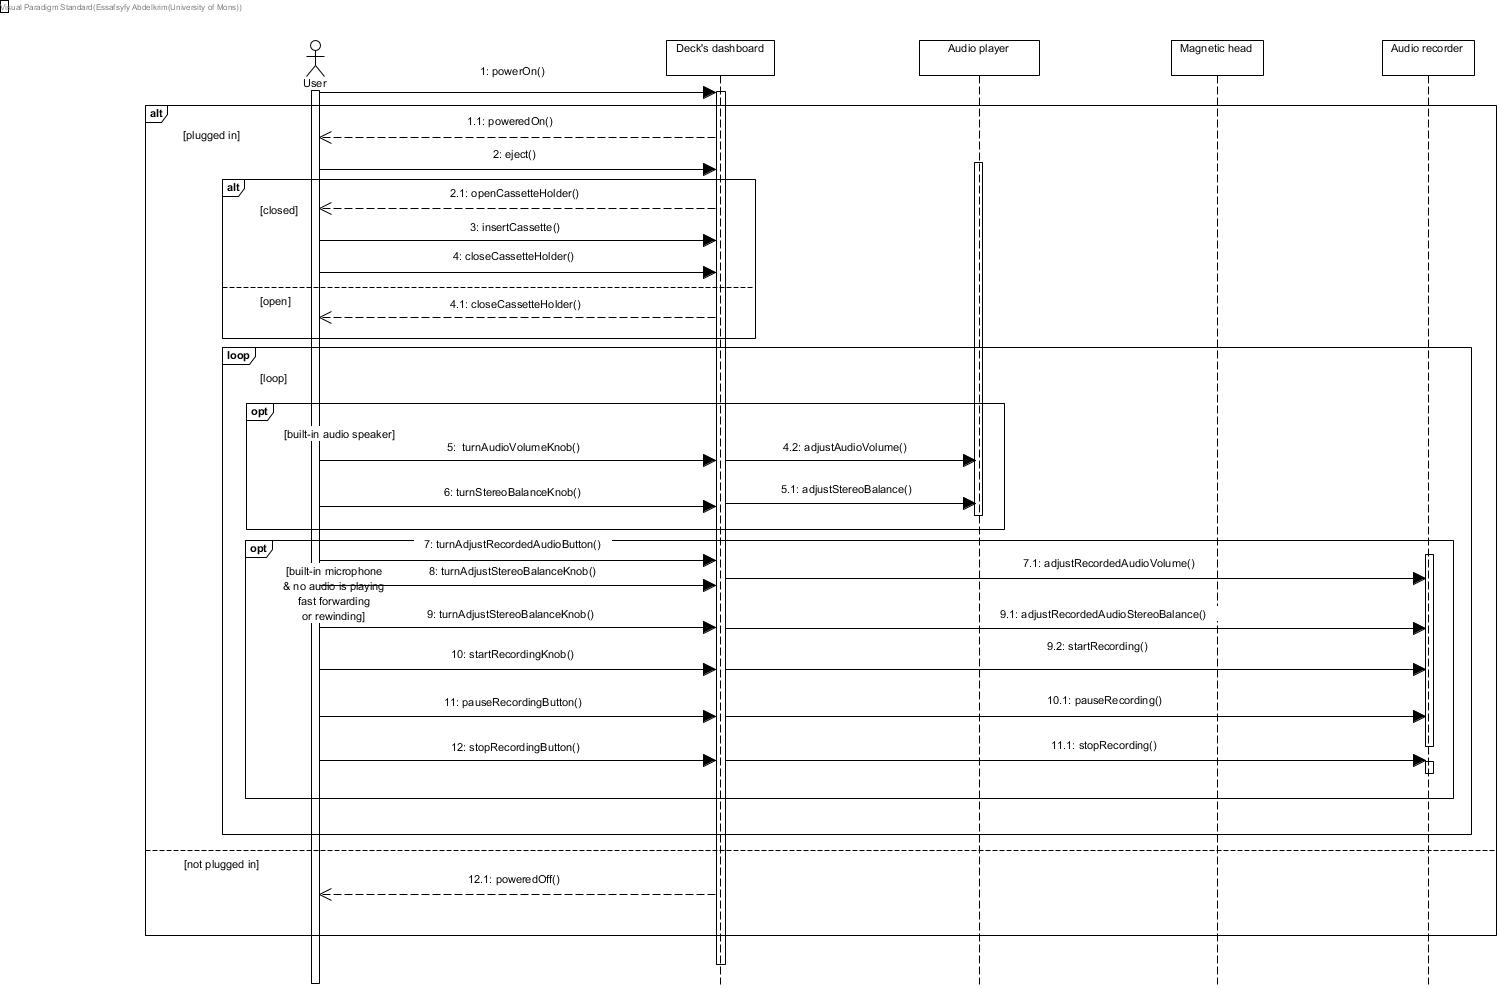
\includegraphics[width=15cm]{./img/musicRecorder(SD).jpg}\\
\end{center}
This diagram describes the steps a user follows to record audio using the deck's audio recorder, provided the former has a built-in microphone. Similar to the Music player diagram, the user has to power on, eject the cassette holder and insert a cassette and finally close the holder to record audio.\\
The User is able to adjust the recorded audio's volume as well as its stereo balance using the respective knob.

\pagebreak
\section{Activity diagram}
\vspace{10px}
\begin{center}
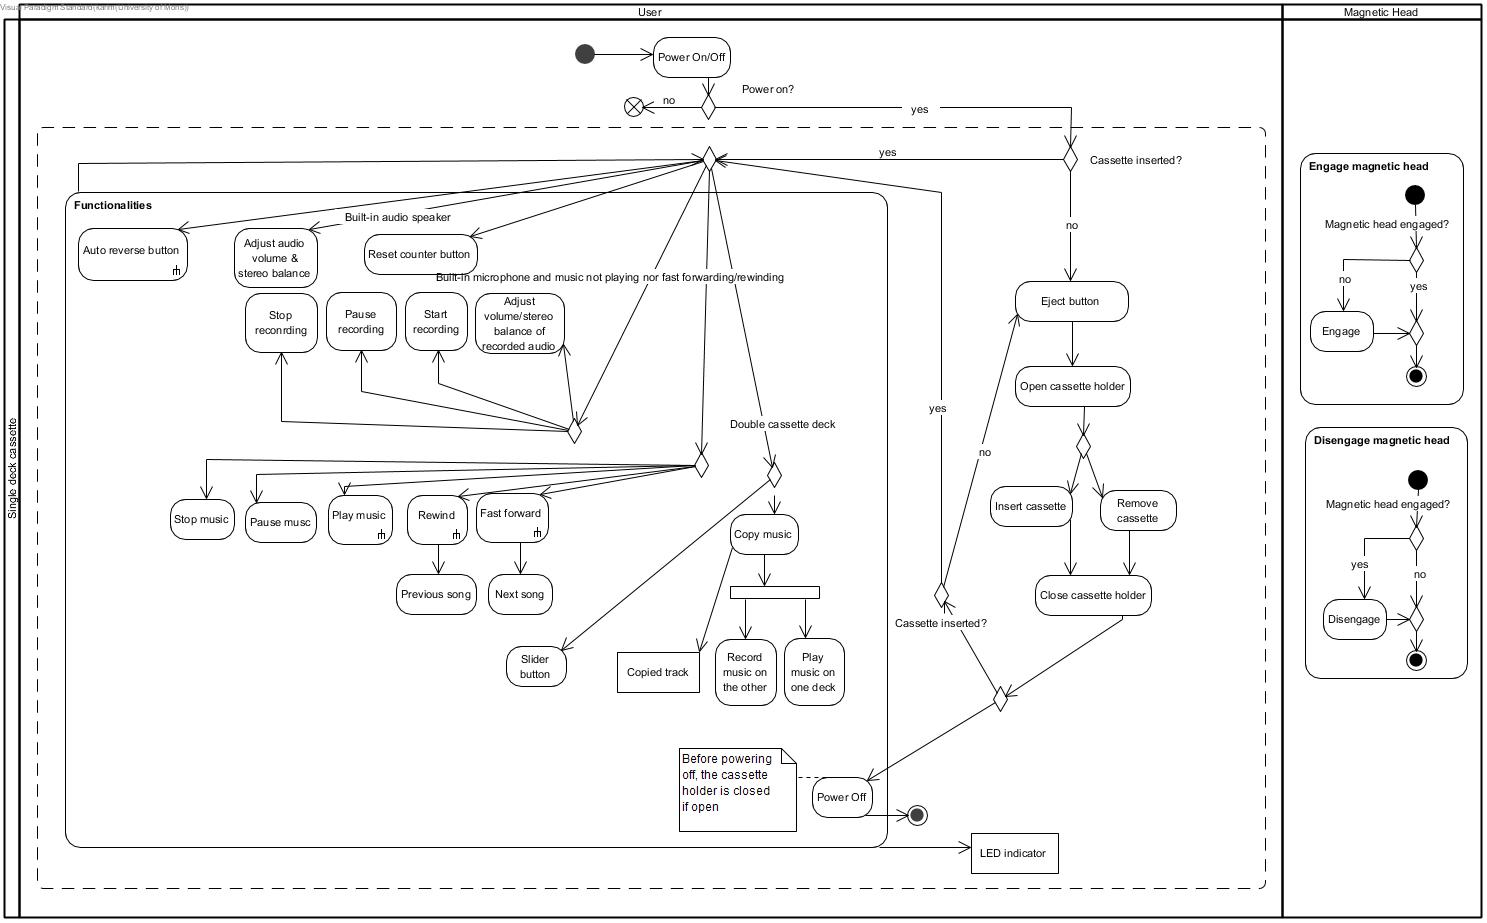
\includegraphics[width=15cm]{./img/activityDiagram_final.jpg}\\
\end{center}
The activity diagram specifies in which order and under what conditions the different cases of the Use case diagram will be executed. For example, the user has to power the deck on in order to perform any operation.\\
Two horizontal \textit{swimlanes} are used to differentiate between the user and the machine's action, in this case, the \textbf{Magnetic Head},  which operates whenever the user performs actions related to the cassette. The \textbf{User} \textit{swimlane} contains the basic course of action to manipulate the deck i.e. ejecting the cassette holder, inserting a cassette, playing it, recording...\\
Some features -such as play, pause, stop...- require the deck's magnetic head to be either engaged or disengaged. To visualize this, a sympbol $\pitchfork$ is used to demonstrate this relation.\\
Furthermore, all operations are assembled in an activity called \textbf{Functionalities}. The latter being recursive, the user can perform these operations over and over again until the \textbf{Power} button is pressed, thus the use of an \textit{interruptible activity region}.


\pagebreak
If need be, a link to the git repository used for this project:\\
\url{https://github.com/Virtuosek/CassetteDeck}

\end{document}